%This work is licensed under the Creative Commons License Attribution 4.0 International (CC-BY 4.0)
%https://creativecommons.org/licenses/by/4.0/legalcode
\documentclass[rgb]{standalone}
\usepackage{tkz-euclide}
\definecolor{myorange}{hsb}{0.0833, 1, 0.8}
\definecolor{mygreen}{hsb}{0.3333, 1, 0.8}
\definecolor{myblue}{hsb}{0.5833, 1, 0.8}
\definecolor{mymagenta}{hsb}{0.8333, 1, 0.8}
\begin{document}
	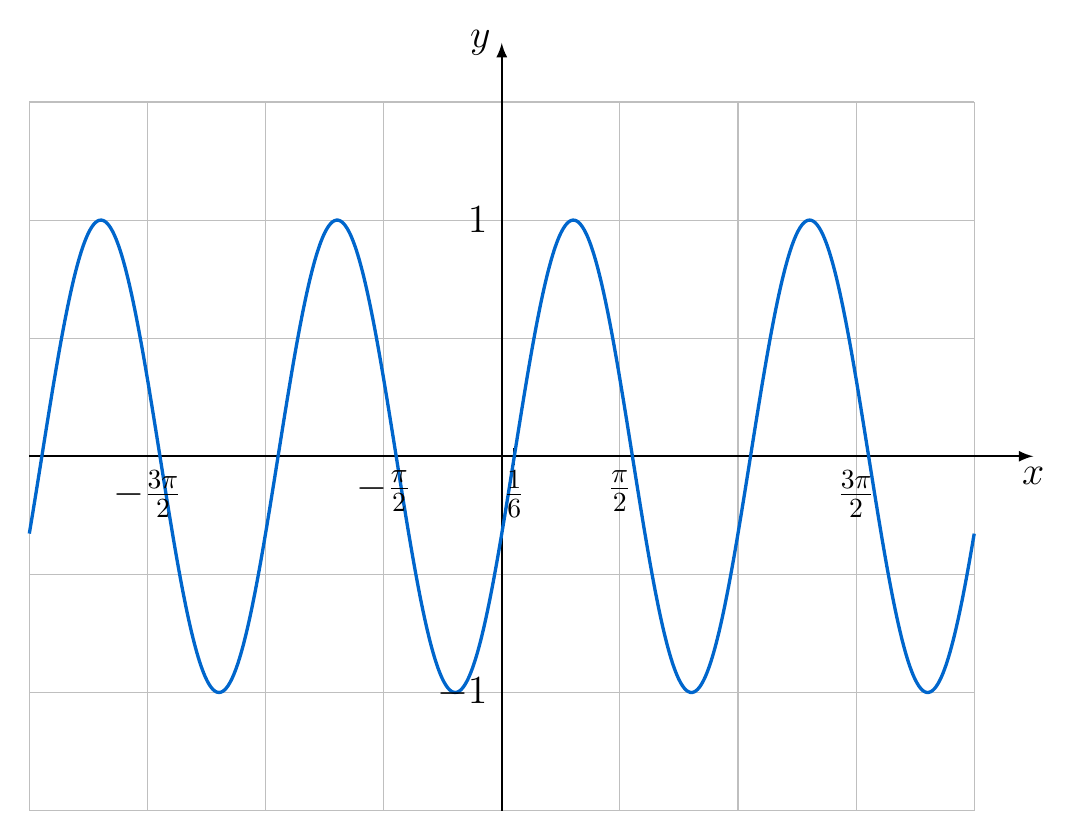
\begin{tikzpicture}[scale=1.5, font=\Large]
		% Coordinate system
		\tkzInit[xmin=-4,xmax=4,ymin=-3,ymax=3]
		\tkzGrid[color=lightgray]
		\tkzDrawX[thick]
		\tkzDrawY[thick]
		\draw[thick] ({1/(3*pi)},-0.07) -- ({1/(3*pi)},0.07);
		\draw[very thick,domain={-30/pi-360}:{360-30/pi}, smooth, samples=500, variable=\x,myblue] plot ({\x/90+1/(3*pi)}, {2*sin(2*\x)});
		\node[below=0.5mm] at (1,0){$\frac{\pi}{2}$};
		\node[below=0.5mm] at ({1/(3*pi)},0){$\frac{1}{6}$};
		\node[below=0.5mm] at (3,0){$\frac{3\pi}{2}$}; 
		\node[below=0.5mm] at (-1,0){$-\frac{\pi}{2}$}; 
		\node[below=0.5mm] at (-3,0){$-\frac{3\pi}{2}$};
		\node[left=0.5mm] at (0,2){$1$};
		\node[left=0.5mm] at (0,-2){$-1$};
	\end{tikzpicture}	
\end{document}